\documentclass[byrevtex,amssymb,aps,pra,floatfix,letterpaper]{revtex4}
\usepackage{graphicx}
\usepackage{hyperref}
\usepackage{verbatim}
\bibliographystyle{apsrev}
\date{\today}
\pagestyle{plain}
\newcommand{\degree}[0]{$^\circ$}

\begin{document}

\title{Experiment 4: Conductivity of electrolyte solutions}

\date{\today}

\maketitle

\section{Introduction}

Pure water does not conduct electricity, but any solvated ionic species would contribute to conduction of electricity. An ionically conducting solution is called an electrolyte solution and the compound, which produces the ions as it dissolves, is called an electrolyte. A strong electrolyte is a compound that will completely dissociate into ions in water. Correspondingly, a weak electrolyte dissolves only partially. The conductivity of an electrolyte solution depends on concentration of the ionic species and behaves differently for strong and weak electrolytes. In this work the electric conductivity of water containing various electrolytes will be studied. The data will be extrapolated to infinitely dilute solutions and the acidity constant for a given weak electrolyte will also be determined. Additional theoretical background for electrolyte solutions can be found from Refs. \cite{ATKINS1,SILBEY,CHANG}.

\section{Theory}

Movement of ions in water can be studied by installing a pair of electrodes into the liquid and by introducing a potential difference between the electrodes. Like metallic conducting materials, electrolyte solutions follow Ohm's law:

\begin{equation}
R = \frac{U}{I}
\label{eq1}
\end{equation}

\noindent
where $R$ is the resistance ($\Omega$, ``ohms''), $U$ is the potential difference (V, ``Volts''), and $I$ is the current (A, ``Amperes''). Conductance $G$ (S, Siemens or $\Omega^{-1}$) is then defined as reciprocal of the resistance:

\begin{equation}
G = \frac{1}{R}
\label{eq2}
\end{equation}

\noindent
Conductance of a given liquid sample decreases when the distance between the electrodes increases and increases when the effective area of the electrodes increases. This is shown in the following relation:

\begin{equation}
G = \kappa\frac{A}{l}
\label{eq3}
\end{equation}

\noindent
where $\kappa$ is the conductivity (S m$^{-1}$), $A$ is the cross-sectional area of the electrodes (m$^2$; i.e., the effective area available for conducting electrons through the liquid), and $l$ is the distance between the electrodes (m). Molar conductivity $\Lambda_m$ (S m$^2$ mol$^{-1}$) is defined as:

\begin{equation}
\Lambda_m = \frac{\kappa}{c}
\label{eq4}
\end{equation}

\noindent
where $c$ is the molar concentration of the added electrolyte. A typical value for molar conductivity is 10 mS m$^2$ mol$^{-1}$.

The molar conductivity of an electrolyte would be independent of concentration if $\kappa$ were proportional to the concentration of the electrolyte. In practice, however, the molar conductivity is found to vary with the concentration (see Fig. \ref{fig1}). One reason for this variation is that the number of ions in the solution might not be proportional to the concentration of the electrolyte. For example, the concentration of ions in a solution of a weak acid depends on the concentration of the acid in a complicated way, and doubling the concentration of the acid does not double the number of ions. Another issue is that ions interact with each other and tend to slow down each other leading reduced conductivity. In this limit, the molar conductivity depends on square root of electrolyte molar concentration.

\begin{figure}[!htp]
\begin{center}
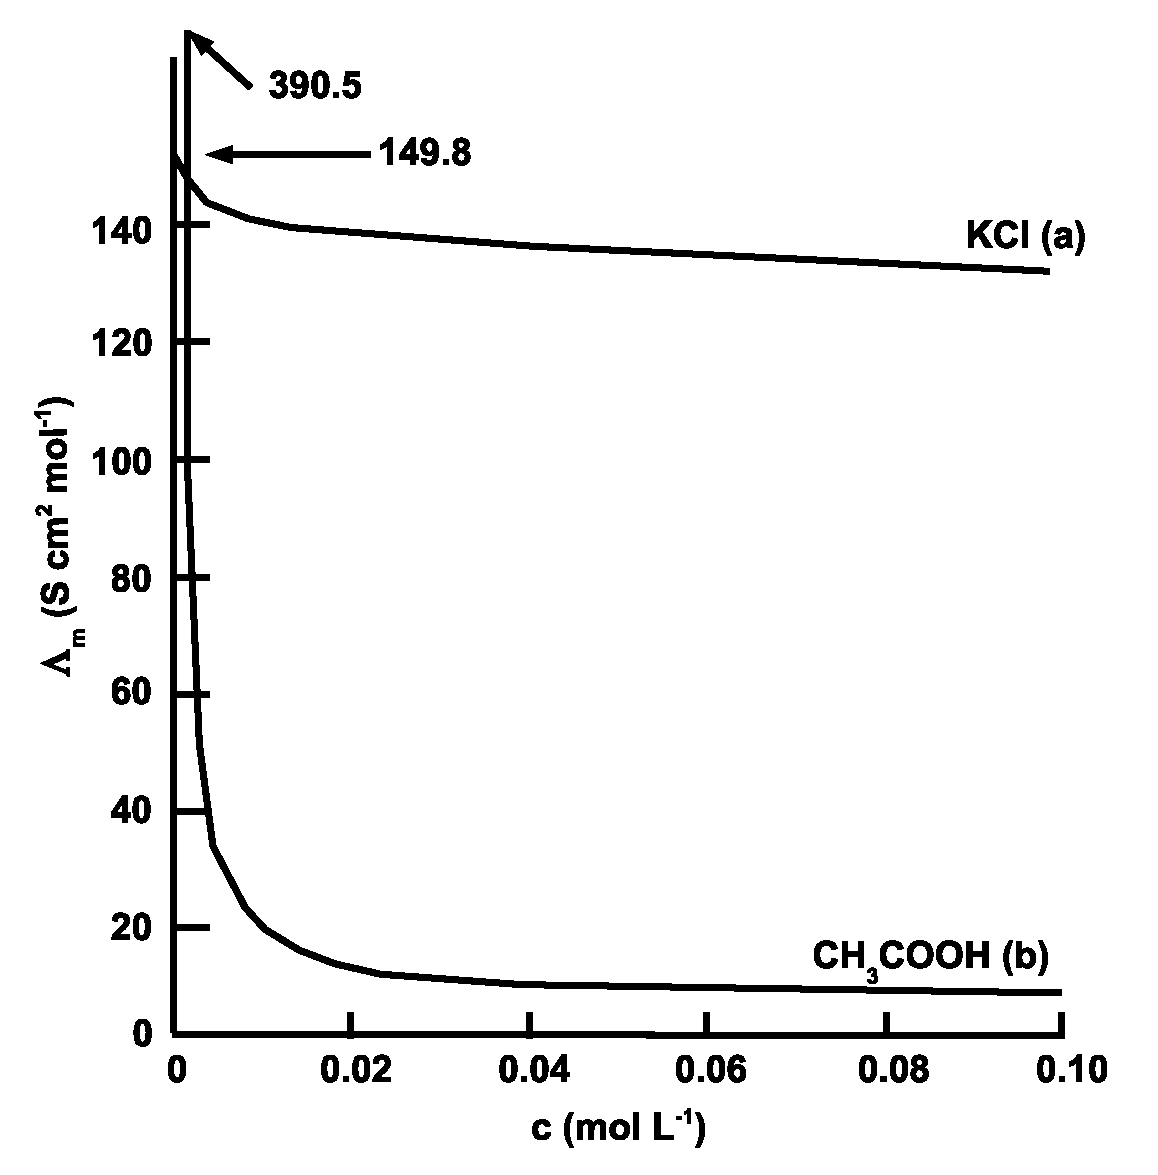
\includegraphics[scale=0.3]{mcond}
\caption{Variation of molar conductivity as a function of molar concentration. a) Strong electrolute and b) weak electrolyte.}
\label{fig1}
\end{center}
\end{figure}

In the 19th century Friedrich Kohlrausch discovered the following empirical relation between the molar concentration of a strong electrolyte and the molar conductivity (Kohlrausch's law) at low concentrations:

\begin{equation}
\Lambda_m = \Lambda_m^0 - K\sqrt{c}
\label{eq5}
\end{equation}

\noindent
where $K$ is a non-negative constant depending on the electrolyte and $\Lambda_m^0$ is the limiting molar conductivity (i.e., the molar conductivity in the limit of zero concentration of the electrolyte). Furthermore, Kohlrausch was able to show that $\Lambda_m^0$ can be expressed as a sum of contributions from its individual ions. If the limiting molar conductivity for the cations is $\lambda_+$ and for the anions $\lambda_-$, the ``law of the independent migration of ions'' states:

\begin{equation}
\Lambda_m^0 = v_+\lambda_+ + v_-\lambda_-
\label{eq6}
\end{equation}

\noindent
where $v_+$ is the number of cations per formula unit, $v_-$ is the corresponding number of anions, and $\lambda_+$ and $\lambda_-$ are the limiting molar conductivities for cations and anions, respectively. For example, for HCl $v_+ = 1$ and $v_- = 1$ but for MgCl$_2$ we have $v_+ = 1$ and $v_- = 2$. Because weak electrolytes are not fully ionized in solution, the number of ions is not proportional to the concentration of the electrolyte but depends on the degree of dissociation ($\alpha$). The \textit{effective} molar conductivity can then be approximated in terms of $\alpha$ and the hypothetical molar conductivity of the fully ionized case ($\Lambda_m^0$):

\begin{equation}
\Lambda_m = \alpha\Lambda_m^0
\label{eq7}
\end{equation}

\noindent
When a weak acid dissociates in water solution, we have:

\begin{equation}
\textnormal{HA}(aq) + \textnormal{H}_2\textnormal{O}(l) \rightleftharpoons \textnormal{H}_3\textnormal{O}^+(aq) + \textnormal{A}^-(aq)
\label{eq8}
\end{equation}

\noindent
The effective concentrations in solution are then given by (subscript 0 refers to the initial concentration of the acid):

\begin{equation}
\left[\textnormal{H}_3\textnormal{O}^+\right] = \alpha\left[\textnormal{HA}\right]_0\textnormal{, }\left[\textnormal{A}^-\right] = \alpha\left[\textnormal{HA}\right]_0\textnormal{, }\left[\textnormal{HA}\right] = \left(1 - \alpha\right)\left[\textnormal{HA}\right]_0
\label{eq9}
\end{equation}

\noindent
The acidity constant ($K_a$) can now be written in terms of the ion activities ($a$):

\begin{equation}
K_a = \frac{a\left(\textnormal{H}_3\textnormal{O}^+\right)a\left(\textnormal{A}^-\right)}{a\left(\textnormal{HA}\right)\underbrace{a\left(\textnormal{H}_2\textnormal{O}\right)}_\textnormal{\tiny = 1 (solvent)}} = \frac{a\left(\textnormal{H}_3\textnormal{O}^+\right)a\left(\textnormal{A}^-\right)}{a\left(\textnormal{HA}\right)}
\label{eq10}
\end{equation}

\noindent
In order to proceed, we write activity in an alternative form for each species (here $i$ = H$_3$O$^+$, A$^-$, HA, H$_2$O):

\begin{equation}
a(i) = \gamma_i\frac{b_i}{b^\theta}
\label{eq11}
\end{equation}

\noindent
where $\gamma_i$ is the activity coefficient (dimensionless) for species $i$, $b_i$ is the molality for $i$ (mol kg$^{-1}$) and $b^\theta$ is the ideal solution molality (constant, 1 mol kg$^{-1}$). Inserting Eq. (\ref{eq11}) into Eq. (\ref{eq10}) we get:

\begin{equation}
K_a = \frac{\gamma_{\textnormal{\tiny H}_3\textnormal{\tiny O}^+}\gamma_{\textnormal{\tiny A}^-}}{\gamma_\textnormal{\tiny HA}} \times \frac{b_{\textnormal{\tiny H}_3\textnormal{\tiny O}}b_{\textnormal{\tiny A}^-}}{b_{\textnormal{\tiny HA}}b^\theta} = K_\gamma\times K_b
\label{eq12}
\end{equation}

\noindent
where notation of $K_\gamma$γ and $K_b$ are used for convenience. Do not confuse $K_b$ with the acidity constant! In dilute solutions the mean activity coefficient ($\gamma_{ave} = \sqrt{\gamma_{\textnormal{\tiny H}_3\textnormal{\tiny O}^+}\gamma_{\textnormal{\tiny A}^-}}$; geometric mean value) can be calculated using the Debye-Hückel limiting law:

\begin{equation}
\log\left(\gamma_{ave}\right) = -\left|z_{\textnormal{\tiny H}_3\textnormal{\tiny O}^+}z_{\textnormal{\tiny A}^-}\right|A\sqrt{I}
\label{eq13}
\end{equation}

\noindent
where $z$'s are the ionic charges, $A$ is a constant (typically 0.509 for an aqueous solution at 25 $^\textnormal{o}$C) and $I$ is the dimensionless ionic strength of the solution given by:

\begin{equation}
I = \frac{1}{2}\sum\limits_{i=1}^{N_{ions}}z_i^2\frac{b_i}{b^\theta}
\label{eq14}
\end{equation}

\noindent
where $N_{ions}$ is the number of difference ionic species in the solution. Note that log here denotes a logarithm with base 10 (ln would denote the natural base logarithm). Since the activity coefficient for the neutral species ($\gamma_\textnormal{\tiny HA}$) is equal to one and $\gamma_{ave}^2 = \gamma_{\textnormal{\tiny H}_3\textnormal{\tiny O}^+}\gamma_{\textnormal{\tiny A}^-}$, the Eq. (\ref{eq12}) gives:

\begin{equation}
K_a = \gamma_{ave}^2\times K_b
\label{eq15}
\end{equation}

\noindent
or by using logarithms:

\begin{equation}
\log\left(K_a\right) = 2\log\left(\gamma_{ave}\right) + \log\left(K_b\right)
\label{eq16}
\end{equation}

\noindent
In dilute solutions molalities are directly related to concentrations by:

\begin{equation}
\left[i\right] = c_i = b_i\rho
\label{eq17}
\end{equation}

\noindent
where $c_i$ is the molar concentration of species $i$ (mol L$^{-1}$; usually denoted by species in brackets) and $\rho$ is the density of the solution (kg L$^{-1}$). Inserting Eq. (\ref{eq17}) into Eq. (\ref{eq16}) we have:

\begin{equation}
\log\left(K_a\right) = 2\log\left(\gamma_{ave}\right) + \log\left(\frac{\left[\textnormal{H}_3\textnormal{O}^+\right]\left[\textnormal{A}^-\right]}{\rho b^\theta\left[\textnormal{HA}\right]}\right)
\label{eq18}
\end{equation}

\noindent
Note that the numerical value of $\rho b^\theta$ is approximately one, so it is only required for getting correct units. In many cases equilibrium constants are written in terms of concentrations, which tends to lead confusion in units. For example, for Eq. (\ref{eq8}) we would normally write in terms of concentration:

\begin{equation}
K_a \approx \frac{\left[\textnormal{H}_3\textnormal{O}^+\right]\left[\textnormal{A}^-\right]}{\left[\textnormal{HA}\right]} =: K_c
\label{eq19}
\end{equation}

\noindent
while this gives the correct magnitude, it gives wrong units as the equilibrium constant is dimensionless (see the definition in Eq. (\ref{eq10})). Variable $K_c$ was introduced to refer to the equilibrium constant obtained directly from concentrations. Thus we can simplify Eq. (\ref{eq18}) as:

\begin{equation}
\log\left(K_a\right) = 2\log\left(\gamma_{ave}\right) + \log\left(\frac{K_c}{\rho b^\theta}\right)
\label{eq20}
\end{equation}

\noindent
From Eqs. (\ref{eq9}) and (\ref{eq19}) $K_c$ can be obtained as:

\begin{equation}
K_c = \frac{\alpha^2\left[\textnormal{HA}\right]_0}{1 - \alpha}
\label{eq21}
\end{equation}

\noindent
Next we apply the Debye-H\"uckel limiting law (Eqs. (\ref{eq13}) and (\ref{eq14})) and Eq. (\ref{eq21}) to Eq. (\ref{eq20}):

\begin{eqnarray}
& & \log\left(K_a\right) = -2\left|z_{\textnormal{\tiny H}_3\textnormal{\tiny O}^+}z_{\textnormal{\tiny A}^-}\right|A\sqrt{I} + \log\left(\frac{K_c}{\rho b^\theta}\right)
= -2A\sqrt{\frac{\alpha\times\left[\textnormal{HA}\right]_0}{\rho b^\theta}} + \log\left(\frac{\alpha^2\left[\textnormal{HA}\right]_0}{\rho b^\theta\left(1 - \alpha\right)}\right)\\
\nonumber
& & \textnormal{OR}\\
& & pK_a = -\log\left(K_a\right) = 2A\sqrt{\frac{\alpha\times\left[\textnormal{HA}\right]_0}{\rho b^\theta}} - \log\left(\frac{\alpha^2\left[\textnormal{HA}\right]_0}{\rho b^\theta(1 - \alpha)}\right)
\nonumber
\label{eq22}
\end{eqnarray}

\noindent
In practice $\alpha$ can be obtained from Eq. (\ref{eq7}). However, before Eq. (\ref{eq7}) can be applied we must know the limiting molar conductivities for solution consisting of H$_3$O$^+$ and A$^-$.

In order to calculate the limiting conductivity mentioned above, we must use Eq. (\ref{eq6}). Note that we cannot use Eq. (\ref{eq5}) since it only applies to strong electrolytes. For the present case Eq. (\ref{eq6}) reads (HA = CH$_3$COOH):

\begin{equation}
\Lambda_m^0(\textnormal{CH}_3\textnormal{COOH}) = \lambda_+(\textnormal{H}_3\textnormal{O}^+) + \lambda_-(\textnormal{CH}_3\textnormal{COOH}^-)
\label{eq23}
\end{equation}

\noindent
Such data is not directly available, but can be calculated, for example, by measuring the limiting molar conductivities of the following strong electrolyte (water) solutions:

\begin{eqnarray}
& \textnormal{HCl} \rightarrow \textnormal{H}_3\textnormal{O}^+ + \textnormal{Cl}^- & (\Lambda_{1,m}^0 = \lambda_+(\textnormal{H}_3\textnormal{O}^+) + \lambda_-(\textnormal{Cl}^-))\\
\nonumber
& \textnormal{NaCl} \rightarrow \textnormal{Na}^+ + \textnormal{Cl}^- & (\Lambda_{2,m}^0 = \lambda_+(\textnormal{Na}^+) + \lambda_-(\textnormal{Cl}^-))\\
\nonumber
& \textnormal{CH}_3\textnormal{COONa} \rightarrow \textnormal{CH}_3\textnormal{COO}^- + \textnormal{Na}^+ & (\Lambda_{3,m}^0 = \lambda_+(\textnormal{Na}^+) + \lambda_-(\textnormal{CH}_3\textnormal{COO}^-))
\label{eq24}
\end{eqnarray}

\noindent
If the three limiting conductivities can be measured then the limiting conductivity for Eq. (\ref{eq23}) is given by:

\begin{equation}
\Lambda_m^0(\textnormal{CH}_3\textnormal{COOH}) = \Lambda_{3,m}^0 - \Lambda_{2,m}^0 + \Lambda_{1,m}^0
\label{eq25}
\end{equation}

\noindent
Thus Eq. (\ref{eq7}) now reads:

\begin{equation}
\alpha = \frac{\Lambda_m(\textnormal{CH}_3\textnormal{COOH})}{\Lambda_m^0(\textnormal{CH}_3\textnormal{COOH})} = \frac{\overbrace{\Lambda_m(\textnormal{CH}_3\textnormal{COOH})}^{\textnormal{\tiny ``to be measured''}}}{\underbrace{\Lambda_{3,m}^0 - \Lambda_{2,m}^0 + \Lambda_{1,m}^0}_{\textnormal{\tiny ``to be determined separately''}}}
\label{eq26}
\end{equation}

\section{Experimental}

\noindent
\underline{Task overview:} Measure conductivities of 0.03 M, 0.02 M, 0.015 M, 0.01M and 0.005 M solutions of three strong electrolytes (NaCl, HCl, CH$_3$CO$_2$Na) and one weak electrolyte (acetic acid; CH$_3$CO$_2$H) using a conductivity meter.\\

\noindent
\underline{Calibration solution:} If calibration solution (0.01 KCl in deionized water) is not available, it can be prepared by weighing 0.3728 g of anhydrous KCl and dissolving it in 500.0 mL of deionized water.\\

\noindent
\underline{Electrolyte solutions:} Prepare 200 mL electrolyte solutions in volumetric flasks. Use the electrolytes and concentrations given in the task overview above. CH$_3$COOH and HCl are given as 0.1 M stock solutions whereas the rest of the compounds are given as solids. Be sure to mix the solutions well before measurement.\\

\noindent
\underline{Measurements:} Use a beaker, which allows full immersion of the electrodes in the solution. Handle the electrode with care and \textbf{be sure to connect the electrode cable to the meter correctly -- otherwise you may damage the instrument!} Always rinse the electrode with deionized water before use. Use a magnetic stirrer to ensure that the solution is homogenous during the measurement. Before taking readings, always shake the electrode briefly to release possible air bubbles trapped in the electrode. First, perform calibration measurement using the 0.01 M KCl-solution. The literature value for conductivity of this solution is 1.413 mS cm$^{-1}$ at 25 $^\textnormal{o}$C. If the readout deviates from this, perform calibration of the conductivity meter (see the manual; \underline{adjust the two RVs for both measurement scales}). Note that the instrument readout units are mS / cm. After calibration, proceed in measuring your electrolyte solutions. Carry out measurements always starting from the most dilute sample and working towards the most concentrated one. When proceeding to a new compound, change the beaker.

\section{Data analysis}

\noindent
1. \underline{Limiting conductivities for strong electrolytes:} Use Eq. (\ref{eq5}) to obtain the limiting molar conductivities ($\Lambda_m^0$) for each strong electrolyte using qtiplot. $\Lambda_m^0$ will be the Y-axis intercept.
\begin{enumerate}
\item Enter the electrolyte concentrations (X) and measured molar conductivities (Y) in table1 in qtiplot. Be sure to use molar conductivities (i.e., use Eq. (\ref{eq4}) to get them) and enter them in standard SI units.
\item Change the X axis to $\sqrt{X}$ by first selecting the X column by clicking at the top of the column by mouse. Then use ``Table $\rightarrow$ Set Column Values...'', enter the following into the large text box: sqrt(col("1")) and finally click on Apply and Close. Note that the square root must be taken according to Eq. (\ref{eq5}).
\item Select the Y column by clicking on the column header by mouse. Then proceed to fitting a straight line to your data by choosing ``Analysis $\rightarrow$ Fit Linear''. The fitted line will now be shown on the graph and the slope and the intercept can be read from the Results.log window. Note that you may have to scroll the window up to see the values. Be sure to record the errors as well as the $r^2$ value for your fit. All graphs along with the obtained fitted values must be included in the laboratory report. Repeat the procedure for each electrolyte (except acetic acid).
\end{enumerate}
The obtained limiting conductivity values (intercepts in the linear fit) are required to calculate $\alpha$ in Eq. (\ref{eq26}) and finally pK$_\textnormal{a}$ for CH$_3$COOH (step 2 below).\\

\noindent
2. \underline{pK$_\textnormal{a}$ of acetic acid:} After determining the limiting conductivities for the strong electrolytes, the conductivity data for acetic acid (weak electrolyte) will be used to determine the pK$_\textnormal{a}$. To do this with qtiplot, carry out the following steps:

\begin{enumerate}
\item Create a table with the concentrations (X) (mol L$^{-1}$) and molar conductivity values (Y) (S m$^2$ mol$^{-1}$) with qtiplot. You can enter these values in table1, which is opened by default when you start the program.
\item Transform your data to get a linear dataset. Create two new columns to your table by choosing ``Table $\rightarrow$ Columns...'' and change the number of columns from 2 to 4. Set column 3 type to X by selecting it first with mouse and then choosing ``Table $\rightarrow$ Set Column As'' and choose X from there. Create the transformed X axis by first selecting the new X column with mouse and then choosing ``Table $\rightarrow$ Set Column Values...'' and enter the following expression in the large input box:

\begin{verbatim}
sqrt(col("1")*col("2")/(XX-YY+ZZ))
\end{verbatim}

where above XX denotes your limiting molar conductivity value for HCl, YY for NaCl, and ZZ for CH$_3$COONa. Click ``Apply'' and ``Close''. Then transform your Y data by first selecting the new Y column, choosing ``Table $\rightarrow$ Set Column Values...'' and enter the following expression into the large input box:

\begin{verbatim}
-log((col("2")/(XX-YY+ZZ))^2 * col("1") / (1 - col("2")/(XX-YY+ZZ)))
\end{verbatim}

Click ``Apply'' and ``Close'' to transform the column. If you made a mistake in entering the expression, you will get an error (or wrong data).

\item Perform a linear fit to your data. Select the new Y colum (Y2) by clicking on the top of the column by mouse. Choose ``Analysis $\rightarrow$ Fit Linear''. The linear fit to your data will be shown on the graph and the slope and the intercept can be read from the Results.log window. Note that you may have to scroll the window up before you can find the values. The output will indicate the slope ($k$) and intercept ($b$) according to:

\begin{equation}
\label{eq27}
\underbrace{-\log\left(\frac{\alpha^2\left[\textnormal{HA}\right]_0}{\rho b^\theta\left(1 - \alpha\right)}\right)}_\textnormal{``y''} = \underbrace{-2A\sqrt{\frac{1}{\rho b^\theta}}}_\textnormal{``k''}\times\underbrace{\sqrt{\alpha\left[\textnormal{HA}\right]_0}}_\textnormal{``x''} + \underbrace{\textnormal{pK}_\textnormal{a}}_\textnormal{``b''}
\end{equation}

\noindent
where, for example, the value of $b$ corresponds directly to pK$_\textnormal{a}$. Note that you can edit the graph axes etc. (see the laboratory manual introduction).

\end{enumerate}

\section{Written laboratory report}

Follow the general instructions for written laboratory reports. In addition, include the requested data in the following section:\\

\noindent
\textit{Results.} This section must include the values and error estimates for the values of $\Lambda^0_m$(NaCl), $\Lambda^0_m$(HCl), $\Lambda^0_m$(CH$_3$COONa), and pK$_\textnormal{a}$ (from least squares analysis). Find also the literature values for these variables (see Ref. \cite{ATKINS1}, for example). Discuss the possible sources of error, if your data deviates significantly from a straight line in any of the fits.

\section{References}

\vspace{-1cm}

\bibliography{../../references}

\end{document}
